\documentclass[UTF8]{article}
\usepackage{graphicx}
\usepackage{subfigure}
\usepackage{amsmath}
\usepackage{makecell}
\usepackage[utf8]{inputenc}
\usepackage[space]{ctex} %中文包
\usepackage{listings} %放代码
\usepackage{xcolor} %代码着色宏包
\usepackage{CJK} %显示中文宏包
\usepackage{float}
\usepackage{diagbox}
\usepackage{bm}
\usepackage{ulem} 
\usepackage{amssymb}
\usepackage{soul}
\usepackage{color}
\usepackage{geometry}
\usepackage{fancybox} %花里胡哨的盒子
\usepackage{xhfill} %填充包, 可画分割线 https://www.latexstudio.net/archives/8245
\usepackage{multicol} %多栏包
\usepackage{enumitem}
%\usepackage{enumerate} %可以方便地自定义枚举标题
\usepackage{multirow} %表格中多行单元格合并
\usepackage{wasysym} %可以使用wasysym里的一堆奇奇怪怪的符号
\usepackage{hyperref} % url
%%%%%%%%%%%%%%%伪代码%%%%%%%%%%%%%%%
\usepackage{amsmath}
\usepackage{algorithm}
\usepackage{algorithmicx}
\usepackage[noend]{algpseudocode}
%%%%%%%%%%%%%%%画图包%%%%%%%%%%%%%%%
\usepackage{tikz}
\usepackage{pgfplots} % http://pgfplots.sourceforge.net/gallery.html
\usetikzlibrary{pgfplots.patchplots} % 拟合支持
\usetikzlibrary{arrows,shapes,automata,petri,positioning,calc} % 状态图支持
\usetikzlibrary{arrows.meta} % 箭头
\usetikzlibrary{shadows} % 阴影支持
\usepackage{forest} % 画树

\geometry{left = 1.5cm, right = 1.5cm, top=1.5cm, bottom=2cm}

\definecolor{mygreen}{rgb}{0,0.6,0}
\definecolor{mygray}{rgb}{0.5,0.5,0.5}
\definecolor{mymauve}{rgb}{0.58,0,0.82}
\lstset{
	backgroundcolor=\color{white}, 
	%\tiny < \scriptsize < \footnotesize < \small < \normalsize < \large < \Large < \LARGE < \huge < \Huge
	basicstyle = \footnotesize,       
	breakatwhitespace = false,        
	breaklines = true,                 
	captionpos = b,                    
	commentstyle = \color{mygreen}\bfseries,
	extendedchars = false,
	frame = shadowbox, 
	framerule=0.5pt,
	keepspaces=true,
	keywordstyle=\color{blue}\bfseries, % keyword style
	language = C++,                     % the language of code
	otherkeywords={string}, 
	numbers=left, 
	numbersep=5pt,
	numberstyle=\tiny\color{mygray},
	rulecolor=\color{black},         
	showspaces=false,  
	showstringspaces=false, 
	showtabs=false,    
	stepnumber=1,         
	stringstyle=\color{mymauve},        % string literal style
	tabsize=4,          
	title=\lstname           
}

%\sum\nolimits_{j=1}^{M}   上下标位于求和符号的水平右端,
%\sum\limits_{j=1}^{M}   上下标位于求和符号的上下处,
%\sum_{j=1}^{M}  对上下标位置没有设定,会随公式所处环境自动调整。

%%%%%%%%%%%%%画图包%%%%%%%%%%%%%
\usepackage{tikz}
%%%%%%%%%%%%%好看的矩形%%%%%%%%%%%%%
\tikzset{
  rect1/.style = {
    shape = rectangle,% 指定样式
    minimum height=2cm,% 最小高度
    minimum width=4cm,% 最小宽度
    align = center,% 文字居中
    drop shadow,% 阴影
  }
}
%%%%%%%%%%%%%画图背景包%%%%%%%%%%%%%
\usetikzlibrary{backgrounds}

%%%%%%%%%%%%%在tikz中画一个顶点%%%%%%%%%%%%%
%%%%%%%%%%%%%#1:node名称%%%%%%%%%%%%%
%%%%%%%%%%%%%#2:位置%%%%%%%%%%%%%
%%%%%%%%%%%%%#3:标签%%%%%%%%%%%%%
\newcommand{\newVertex}[3]{\node[circle, draw=black, line width=1pt, scale=0.8] (#1) at #2{#3}}
%%%%%%%%%%%%%在tikz中画一条边%%%%%%%%%%%%%
\newcommand{\newEdge}[2]{\draw [black,very thick](#1)--(#2)}
%%%%%%%%%%%%%在tikz中放一个标签%%%%%%%%%%%%%
%%%%%%%%%%%%%#1:名称%%%%%%%%%%%%%
%%%%%%%%%%%%%#2:位置%%%%%%%%%%%%%
%%%%%%%%%%%%%#3:标签内容%%%%%%%%%%%%%
\newcommand{\newLabel}[3]{\node[line width=1pt] (#1) at #2{#3}}

%%%%%%%%%%%%%强制跳过一行%%%%%%%%%%%%%
\newcommand{\jumpLine} {\hspace*{\fill} \par}
%%%%%%%%%%%%%关键点指令,可用itemise替代%%%%%%%%%%%%%
\newcommand{\keypoint}[2]{$\bullet$\textbf{#1}\quad#2\par}
%%%%%%%%%%%%%<T>平均值表示%%%%%%%%%%%%%
\newcommand{\average}[1]{\left\langle #1\right\rangle }
%%%%%%%%%%%%%表格内嵌套表格%%%%%%%%%%%%%
\newcommand{\tabincell}[2]{\begin{tabular}{@{}#1@{}}#2\end{tabular}}
%%%%%%%%%%%%%大黑点item头%%%%%%%%%%%%%
\newcommand{\itemblt}{\item[$\bullet$]}
%%%%%%%%%%%%%大圈item头%%%%%%%%%%%%%
\newcommand{\itemc}{\item[$\circ$]}
%%%%%%%%%%%%%大星星item头%%%%%%%%%%%%%
\newcommand{\itembs}{\item[$\bigstar$]}
%%%%%%%%%%%%%右▷item头%%%%%%%%%%%%%
\newcommand{\itemrhd}{\item[$\rhd$]}
%%%%%%%%%%%%%定义为%%%%%%%%%%%%%
\newcommand{\defas}{=_{df}}
%%%%%%%%%%%%%偏导%%%%%%%%%%%%%
\newcommand{\partialx}[2]{\frac{\partial #1}{\partial #2}}
%%%%%%%%%%%%%蕴含%%%%%%%%%%%%%
\newcommand{\imp}{\rightarrow}
%%%%%%%%%%%%%上取整%%%%%%%%%%%%%
\newcommand{\ceil}[1]{\lceil#1\rceil}
%%%%%%%%%%%%%下取整%%%%%%%%%%%%%
\newcommand{\floor}[1]{\lfloor#1\rfloor}

%%%%%%%%%%%%%双线分割线%%%%%%%%%%%%%
\newcommand*{\doublerule}{\hrule width \hsize height 1pt \kern 0.5mm \hrule width \hsize height 2pt}
%%%%%%%%%%%%%双线中间可加东西的分割线%%%%%%%%%%%%%
\newcommand\doublerulefill{\leavevmode\leaders\vbox{\hrule width .1pt\kern1pt\hrule}\hfill\kern0pt }
%%%%%%%%%%%%%左大括号%%%%%%%%%%%%%
\newcommand{\leftbig}[1]{\left\{\begin{array}{l}#1\end{array}\right.}
%%%%%%%%%%%%%矩阵%%%%%%%%%%%%%
\newcommand{\mat}[2]{\left[\begin{array}{#1}#2\end{array}\right]}
%%%%%%%%%%%%%可换行圆角文本框%%%%%%%%%%%%%
\newcommand{\ovalboxn}[1]{\ovalbox{\tabincell{l}{#1}}}
%%%%%%%%%%%%%设置section的counter, 使从1开始%%%%%%%%%%%%%
\setcounter{section}{0}

%%%%%%%%%%%%%Colors%%%%%%%%%%%%%
\newcommand{\lightercolor}[3]{% Reference Color, Percentage, New Color Name
    \colorlet{#3}{#1!#2!white}
}
\newcommand{\darkercolor}[3]{% Reference Color, Percentage, New Color Name
    \colorlet{#3}{#1!#2!black}
}
\definecolor{aquamarine}{rgb}{0.5, 1.0, 0.83}
\definecolor{Seashell}{RGB}{255, 245, 238} %背景色浅一点的
\definecolor{Firebrick4}{RGB}{255, 0, 0}%文字颜色红一点的
\lightercolor{gray}{20}{lgray}
\newcommand{\hlg}[1]{
	\begingroup
		\sethlcolor{lgray}%背景色
		\textcolor{black}{\hl{\mbox{#1}}}%textcolor里面对应文字颜色
	\endgroup
}



\title{人工智能基础 HW8}
\author{PB18111697 王章瀚}

\begin{document}
\maketitle
\section*{14.12}
\noindent \textbf{Two astronomers in different parts of the world make measurements $M_1$ and $M_2$ of the number of stars $N$ in some small region of the sky, using their telescopes. Normally, there is a small possibility $e$ of error by up to one star in each direction. Each telescope can also (with a much smaller probability $f$) be badly out of focus (events $F_1$ and $F_2$), in which case the scientist will undercount by three or more stars (or if $N$ is less than 3, fail to detect any star at all). Consider the three networks shown in Figure 14.22}

\begin{figure}[H]
	\centering
	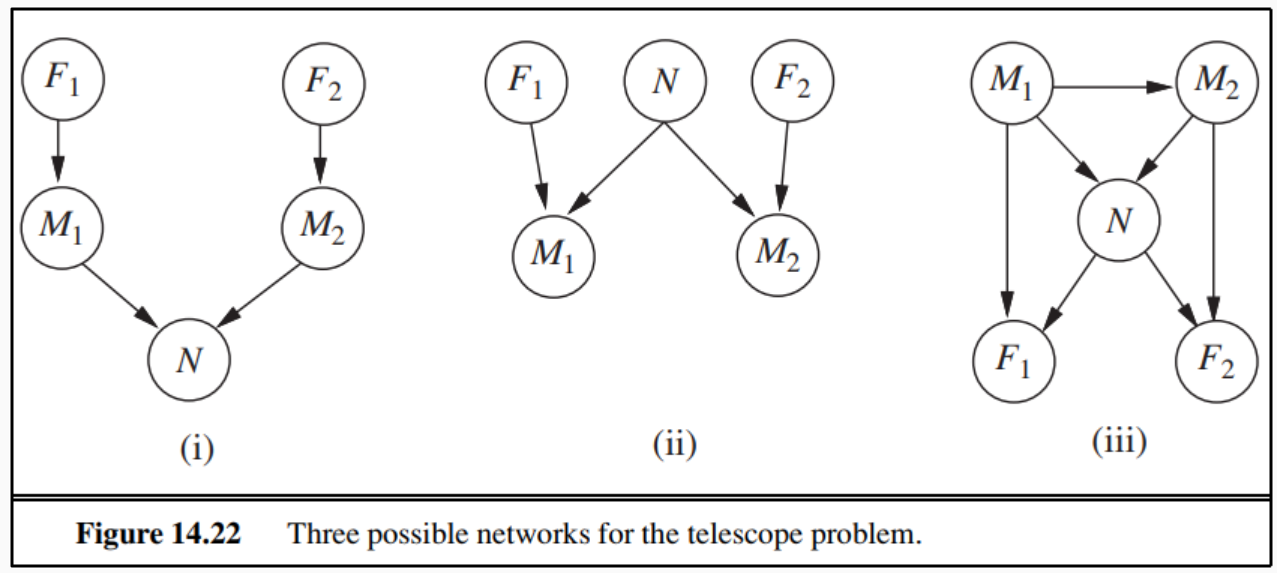
\includegraphics[width=\linewidth*2/3]{image/14.22.png}
\end{figure}\par

\subsection*{a.}
\noindent \textbf{Which of these Bayesian networks are correct (but not necessarily efficient) representations of the preceding information?} \\\jumpLine\noindent
(ii) 是最佳的, 因为 $M_1$ 确实由星星数量 $N$ 和 $F_1$ 所影响, 而 $M_2$ 确实由星星数量 $N$ 和 $F_2$ 所影响. (i) 显然是有问题的, 当给定 $M_1$ 和 $M_2$, 不可能 $F_1$ 和 $F_2$ 就对 $N$ 无影响. (iii) 是按照 $M_1, M_2, N, F_1, F_2$ 的顺序排出的, 没有问题.

\subsection*{b.}
\noindent \textbf{Which is the best network? Explain.} \\\jumpLine\noindent
(ii) 是最佳的. 它结构相对简单, 且准确描述了问题.

\subsection*{c.}
\noindent \textbf{Write out a conditional distribution for $P(M_1|N)$, for the case where $N\in 1,2,3$, and  $M_1\in 0,1,2,3,4$. Each entry in the conditional distribution should be expressed as a function of the parameters $e$ and/or $f$.} \\\jumpLine\noindent
依题意知: 
\begin{align*}
	P(M_1|N) &= P(M_1|N,F_1)P(F_1) + P(M_1|N,\lnot F_1)P(\lnot F_1) \\
\end{align*}
假设少数和多数一颗概率是 $e$, 不多不少是 $1-2e$. 那么可以列表如下:
\begin{center}
	\begin{tabular}{|c|c|c|c|}
		\hline
		\diagbox{$M_1$}{$N$} & 1 & 2 & 3  \\
		\hline
		0 & $f + e(1-f)$ & $f$ & $f$ \\
		\hline
		1 & $(1-2e)(1-f)$ & $e(1-f)$ & $0$ \\
		\hline
		2 & $e(1-f)$ & $(1-2e)(1-f)$ & $e(1-f)$ \\
		\hline
		3 & $0$ & $e(1-f)$ & $(1-2e)(1-f)$ \\
		\hline
		4 & $0$ & $0$ & $e(1-f)$ \\
		\hline
	\end{tabular}
\end{center}

\subsection*{d.}
\noindent \textbf{Suppose $M_1=1$ and $M_2=3$. What are the possible numbers of stars if you assume no prior constraint on the values of $N$ ?} \\\jumpLine\noindent
可能因失焦少了 3 颗, 或因数错多了 $\pm 1$颗. 因此由 $M_1=1$ 知道 $N \in \{0,1,2,4,5,\cdots\}$; 由 $M_2=3$ 知道 $N \in \{2,3,4,6,7,\cdots\}$. $N$ 的可能值必然是二者交集. 故 $N$ 可能为 $\{2,4\}\cup \{6,7,8,9,\cdots\}$.

\subsection*{e.}
\noindent \textbf{What is the most \textit{likely} number of stars, given these observations? Explain how to compute this, or if it is not possible to compute, explain what additional information is needed and how it would affect the result.} \\\jumpLine\noindent
假设 $p_2=P(N=2)$, $p_4=P(N=4)$, $p=P(N>=6)$, 那么
\begin{itemize}
	\item $P(N=2|M_1=1,M_2=3)
	=\frac{P(N=2,M_1=1,M_2=3)}{P(M_1=1, M_2=3)}
	=\frac{p_2e(1-f)e(1-f)}{P(M_1=1, M_2=3)}=\frac{P(N=2,M_1=1,M_2=3)}{P(M_1=1, M_2=3)}
	=\frac{p_2e^2(1-f)^2}{P(M_1=1, M_2=3)}$
	\item $P(N=4|M_1=1,M_2=3)
	=\frac{P(N=4,M_1=1,M_2=3)}{P(M_1=1, M_2=3)}
	=\frac{p_4(1-2e)fe(1-f)}{P(M_1=1, M_2=3)}
	=\frac{p_4e(1-2e)f(1-f)}{P(M_1=1, M_2=3)}$
	\item $\forall k \ge 6$, 
	$P(N=k|M_1=1,M_2=3)
	=\frac{P(N=k,M_1=1,M_2=3)}{P(M_1=1, M_2=3)}
	=\frac{pf^2}{P(M_1=1, M_2=3)}$
\end{itemize}
由于 $f\ll e$, 显然上述三个概率最大的是 $P(N=2|M_1=1,M_2=3)$. 因此 $N=2$ 是最有可能的.

\section*{14.13}
\noindent \textbf{Consider the network shown in Figure 14.22(ii), and assume that the two telescopes work identically. $N\in 1,2,3$, and $M_1,M_2\in 0,1,2,3,4$, with the symbolic CPTs as described in Exercise 14.12. Using the enumeration algorithm (Figure 14.9 on page 525), calculate the probability distributio $P(N|M_1=2,M_2=2)$}

\begin{figure}[H]
	\centering
	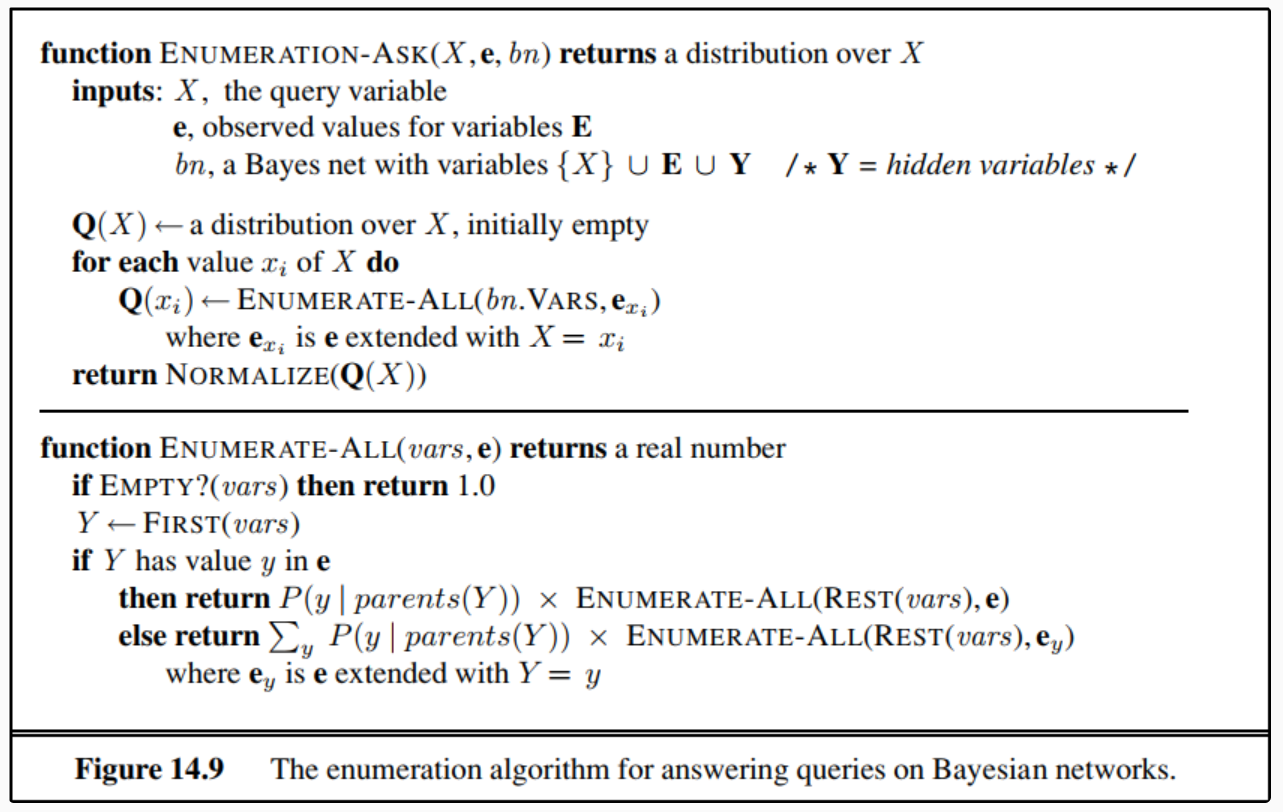
\includegraphics[width=\linewidth*2/3]{image/14.9.png}
\end{figure} \jumpLine\noindent
有变量 $\{N,M_1,M_2,F_1,F_2\}$, 可计算如下:
\begin{align*}
	P(N|M_1=2,M_2=2) &= \alpha\sum\limits_{f_1}\sum\limits_{f_2}P(N, M_1=2, M_2=2,f_1,f_2) \\
	&= \alpha\sum\limits_{f_1}\sum\limits_{f_2}P(N)P(f_1)P(f_2)P(M_1=2|f_1, N)P(M_2=2|f_2, N)
\end{align*}
由于若 $f_1=true$ 或 $f_2=true$ 时对应项 $M_i$ 都不可能达到 2 个星星, 因此只要考虑 $f_1=f_2=false$, 故
$$P(N|M_1=2,M_2=2) = \alpha P(N)(1-f)^2P(M_1=2|false,N)P(M_2=2|false,N)$$
故有 $$P(N=k|M_1=2,M_2=2)=\left\{
\begin{array}{ll}
	\alpha P(N=1)(1-f)^2e^2 & k=1 \\
	\alpha P(N=2)(1-f)^2(1-2e)^2 & k=2 \\
	\alpha P(N=3)(1-f)^2e^2 & k=3 \\
\end{array}
\right.$$



\end{document}




